\documentclass[]{article}
\usepackage{lmodern}
\usepackage{amssymb,amsmath}
\usepackage{ifxetex,ifluatex}
\usepackage{fixltx2e} % provides \textsubscript
\ifnum 0\ifxetex 1\fi\ifluatex 1\fi=0 % if pdftex
  \usepackage[T1]{fontenc}
  \usepackage[utf8]{inputenc}
\else % if luatex or xelatex
  \ifxetex
    \usepackage{mathspec}
  \else
    \usepackage{fontspec}
  \fi
  \defaultfontfeatures{Ligatures=TeX,Scale=MatchLowercase}
\fi
% use upquote if available, for straight quotes in verbatim environments
\IfFileExists{upquote.sty}{\usepackage{upquote}}{}
% use microtype if available
\IfFileExists{microtype.sty}{%
\usepackage{microtype}
\UseMicrotypeSet[protrusion]{basicmath} % disable protrusion for tt fonts
}{}
\usepackage[margin=1in]{geometry}
\usepackage{hyperref}
\hypersetup{unicode=true,
            pdftitle={Identifying copy number alteration using CBS},
            pdfborder={0 0 0},
            breaklinks=true}
\urlstyle{same}  % don't use monospace font for urls
\usepackage{graphicx,grffile}
\makeatletter
\def\maxwidth{\ifdim\Gin@nat@width>\linewidth\linewidth\else\Gin@nat@width\fi}
\def\maxheight{\ifdim\Gin@nat@height>\textheight\textheight\else\Gin@nat@height\fi}
\makeatother
% Scale images if necessary, so that they will not overflow the page
% margins by default, and it is still possible to overwrite the defaults
% using explicit options in \includegraphics[width, height, ...]{}
\setkeys{Gin}{width=\maxwidth,height=\maxheight,keepaspectratio}
\IfFileExists{parskip.sty}{%
\usepackage{parskip}
}{% else
\setlength{\parindent}{0pt}
\setlength{\parskip}{6pt plus 2pt minus 1pt}
}
\setlength{\emergencystretch}{3em}  % prevent overfull lines
\providecommand{\tightlist}{%
  \setlength{\itemsep}{0pt}\setlength{\parskip}{0pt}}
\setcounter{secnumdepth}{0}
% Redefines (sub)paragraphs to behave more like sections
\ifx\paragraph\undefined\else
\let\oldparagraph\paragraph
\renewcommand{\paragraph}[1]{\oldparagraph{#1}\mbox{}}
\fi
\ifx\subparagraph\undefined\else
\let\oldsubparagraph\subparagraph
\renewcommand{\subparagraph}[1]{\oldsubparagraph{#1}\mbox{}}
\fi

%%% Use protect on footnotes to avoid problems with footnotes in titles
\let\rmarkdownfootnote\footnote%
\def\footnote{\protect\rmarkdownfootnote}

%%% Change title format to be more compact
\usepackage{titling}

% Create subtitle command for use in maketitle
\newcommand{\subtitle}[1]{
  \posttitle{
    \begin{center}\large#1\end{center}
    }
}

\setlength{\droptitle}{-2em}
  \title{Identifying copy number alteration using CBS}
  \pretitle{\vspace{\droptitle}\centering\huge}
  \posttitle{\par}
  \author{}
  \preauthor{}\postauthor{}
  \date{}
  \predate{}\postdate{}


\begin{document}
\maketitle

\subsubsection{Background: Why are we looking at copy
number}\label{background-why-are-we-looking-at-copy-number}

DNA copy number refers to the abundancy of a small piece of chomosome,
and is of both biological and medical interests. Cancer initiation is
often associated with accumulated DNA mutation followed by DNA
alteration at a larger scale, because of the inefficiency of DNA
repairing mechanism. Copy numeval.after = c(`fig.cap',`code'),ber
alteration can also be observed in germline cells, often associated with
genetic diseases. Hence, reliable detection of copy number alteration
would enable non-invasive cancer diagnosis and screens for genetic
diseases. It also serves as an intermediate between chromosome
morphology analysis and sequencing analysis, often conducted through
microarray.

\begin{figure}
\centering
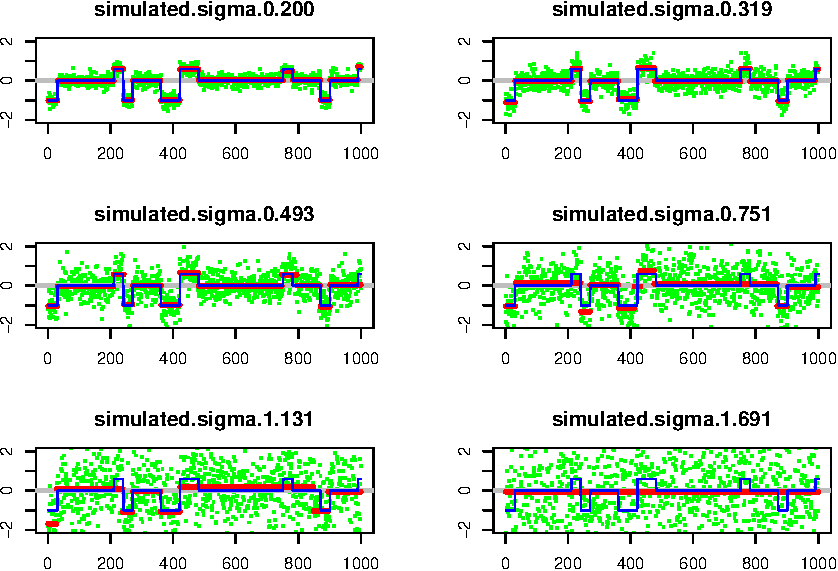
\includegraphics{copynumber_files/figure-latex/CBS-1.pdf}
\caption{\label{fig:CBS_1} CBS result for different noise level. Green:
raw probe response; Blue: theoretical model; Red: CBS segmentation}
\end{figure}

\paragraph{Data simulation}\label{data-simulation}

The data is simulated by concatenating a sample of segments. The
copy-number of the segments follows a multinomial distribution, whereas
their length follows Poisson distribution (\cite instruction ). At the
end an artificial chromosome of 200Mbp is generated, as represented by
30K equally-spaced probe, giving an inter-probe distance of appx. 6kbp.
We experimented with different parameters of \(L_{loss}\),
\(L_{dup}\),\(L_{norm}\), \(p_{loss}\), \(p_{dup}\), \(p_{norm}\), and
selected a parameter set that generated aberrations that span around
\(10^2\) probes so that there is enough signal to perform CBS
segmentation, while keeping the ``normal'' to be the longest and most
likely segment type. The parameters read:

\[
\begin{aligned}
L_{loss} = 20\cdot 10^4bp\\
L_{norm} = 60\cdot 10^4bp\\
L_{dup}  = 20\cdot 10^4bp\\
p_{loss} = 0.25 \\
p_{norm}= 0.5\\
p_{dup}  = 0.25\\
\end{aligned}
\] Each probe is then assigned a copy-number response of 1/2/3 according
to its segment. The response is log-transformed into logR and masked
with a gaussian noise \[
\begin{aligned}
logR = \log_{2}(R/2) + \epsilon \\
\epsilon \sim N(0, \sigma^2)
\end{aligned}
\]

\paragraph{Segmentation under noise}\label{segmentation-under-noise}

Segmentation is performed on the observed logR with DNACopy (1) , for
different \(\sigma\). For each dataset, we calculated
mean\_absolute\_error between the fitted response and the theoretical
model according to eq(1) to evaluate the quality of the fit. As noise
becomes more prevalent, the prediction becomes less reliable (see figure
\ref{fig:contam_stat} and \ref{fig:CBS_1}). Note the
mean\_absolute\_error needs to be compared against a completely null
prediction, that is, the expected error if no segment is predictied.
(mean\_absolute\_error=0.179). For example, at sigma=1.691, the MAE
appears worse than not predicting any copy number changes.

\begin{enumerate}
\def\labelenumi{(\arabic{enumi})}
\tightlist
\item
  \[
  MAE=\frac{\sum_{probe}{|logR(probe)-logR_M(probe)}|}{N(probe)}
  \] where \(logR_M\) denotes the logR from theoretical model, \(logR\)
  denotes that from the observed probe response.
\end{enumerate}

\paragraph{Calling copy numbers}\label{calling-copy-numbers}

In order to define regions with DNA losses, we first attempted a simple
thresholding algorithm, where segment means are compared against a fixed
threshold, below which the segment is declared to have underwent a
``loss'' event. To compare the merit of different thresholds, we plotted
Precision-Recall curve for different thresholds under all noise levels.

To simplify the evaluation, we ignored the segments for now and compute
on a per-probe basis. A model is binariesd with
``\(logR_M(probe) == -1.0\)'', whereas a prediction is binarised with
``\(logR(probe) < threshold\)'', which are then combined to calculate
TP,FP,TN,FN, and converted into precision and recall (eq(2)). The use of
PR curve is justified by the imbalanced nature of the sample.

\begin{enumerate}
\def\labelenumi{(\arabic{enumi})}
\setcounter{enumi}{1}
\tightlist
\item
  \[
  \begin{aligned}
  Precision &: P = \frac{TP}{TP+FP} \\
  Recall &: R = \frac{TP}{TP+FN}
  \end{aligned}
  \]
\end{enumerate}

\[
\begin{aligned}
TN = N( model = 1) \\ 
\leftrightarrow TN = N( \log_2{(model/2)} = -1) \\ 
TN + FP = N(fitted < threshold)
\end{aligned}
\]

As can be seen from the PR-curve ( figure \ref{fig:eval_thres}), it is
possible to achieve P=1 and R=1 for less noisy data, whereas some
trade-off is necessary in treating noisy data. The question then becomes
how to find the sweet spot without referencing the actual model. This
must involves some calculation on the observation side, e.g by looking
at the distribution of fitted segment means.

\begin{figure}
\centering
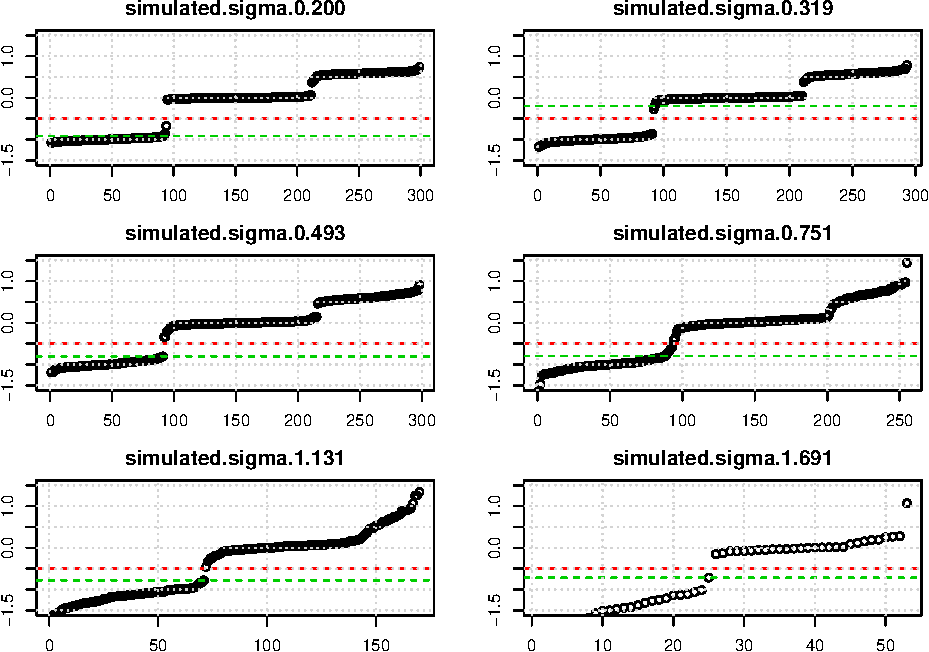
\includegraphics{copynumber_files/figure-latex/DEBUG__seg_thres-1.pdf}
\caption{\label{fig:DEBUG_thres} Sorted segmented means. Red: threshold
= -0.5; Green: threshold by cluster}
\end{figure}

The distribution of segment means follow a nice multimodal trend (see
figure). Intuitively, optimal threshold should be placed at where the
value jumps discontinously. This jump is easy to identify manually, and
here we apply a simple gaussian/t-test based clustering to demarcate
such discontinous jumps. The clustering algorithm works as follows: we
start with an empty vector, and add the segment means one by one from
the smallest. Once the vector size reach 5, we start to estimate mean
and standard deviation (using MAD as estimator) from the sample defined
by the vector, so as to estimate the likelihood of the incoming element
to belong to this sample. If the incoming value is significantly
deviating from the sample (using a Z-score cutoff), then this sample is
dumped as a cluster and we start with an empty vector again. As a
result, the whole distribution is segmented into multiple homogeneous
normal distributions.

The resultant clusters are then subject to a one-tail t-test with the
alternative hypothesis that \(\mu < -0.5\), and the cluster is retained
only if there is significant evidence to reject the null
(P\textless{}0.001). In other words, we threshold segment means on a
pre-cluster basis to ensure the consistency of thresholding. As shown in
the PR-curve (figure \ref{fig:thres_eval}), using the selected threshold
we achieved precision \textgreater{} 90\% at all tested level of noises.
Moreover, in cases where a smooth elbow is present, it is always
identified by the cluster-based threshold, achieving the best possible
compromise between precision and recall.

Unlike result from simple thresholding at -0.5, the cluster-based result
always sits on the start of the elbow, does not suffer from the
precision reduction due to noise.

For furture reference, this segmentation algorithm requires several
parameters: (1) MIN\_LEN: is the smallest sample size for a standard
deviation to be estimated (2) Z\_MIN: is the z-score cutoff to declare
the ending of a cluster.(3) SUPER\_THRES: is the prior belief of where
the cutoff lies.

\begin{figure}
\centering
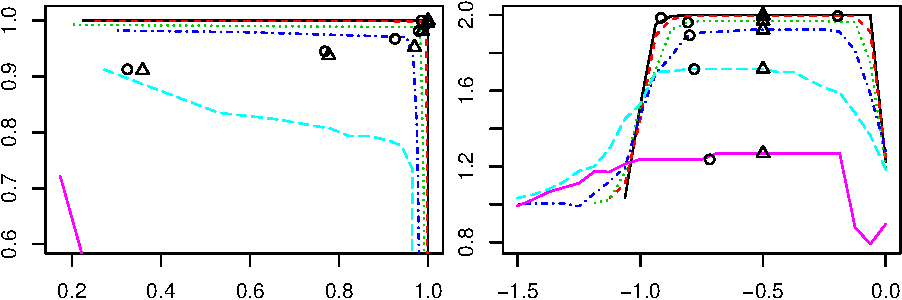
\includegraphics{copynumber_files/figure-latex/plot__PR-1.pdf}
\caption{\label{fig:eval_thres} Evaluation of different threshold.
Circle: Thresholded by cluster. Triangle: Naive thresholding (This plot
is somehow broken after switching dataset)}
\end{figure}

\subsubsection{3. Impact of mixing a normal cell
population}\label{impact-of-mixing-a-normal-cell-population}

We consider a normal cell contamination that attenuates our signal, so
that (@eq01) \[
\begin{aligned}
R_{cM}(probe) &= c \cdot 2 + (1-c) \cdot R_M(probe) \\
\log_{2}{(R_{cM}(probe)/2)} &= \log_{2}{(c+(1-c)\cdot R_M(probe) / 2)}
\end{aligned}
\]

We plotted \(R_{cM}(probe)\) w.r.t. \(R_M(probe)\) on a log-log scale,
showing a approximately linear trend near R(probe)=2, indicating that
the mapped signals should still be separable, albeit less tolerant to
noise. In other words, during outlier-based clustering, SUPER\_THRES
needs to be set dynamically considering the possibility of
contamination, rather than fixed at -0.5.

Firstly, To understand the effect of a normal cell contamination, we
plotted noise-MAE curve for 6 contamination level. Indeed, samples with
higher contamination are more prone to noise (see figure
\ref{fig:contam_stat}).

Secondly, in order to infer this ratio of contamination, we compute the
mean absolute error (MAE, also known as the L1-norm) for a range of
candidate contamination ratio and select the one with the least MAE.
This is done by calculating the average for distances from predicted
segment mean to their most probable copy-number given a candidiate
contamination ratio ( eq(@eq01) for \(R(probe) \in \{1,2,3\}\) ) . It
appears that as contamination increases, the algorithm tends to
under-estimate the ratio (figure \ref{fig:contam_est}), conceivably due
to less segments being available to support the inference.

For summary, we compared 5 threshold estimating scheme on the PR-curve:
(1) Naive thresholding at -0.5 (2) Naive thresholding using theoretical
contamination (3) Cluster-based thresholding at -0.5 (4) Cluster-based
thresholding using theoretical contamintaion (5) Cluster-based
thresholding using guessed contamination

From the summarizing plot, we observe that thresholding using
theoretical contamination reasonably improved the result (type2, type4,
as compared to type1, type3). However, due to the difficulty in
inferring the contamination, it is not always possible to perfrom type5
reliably.

In other words, the putative ``loss'' clusters are shifted towards the
neutral signal, with their shape invaried.

\begin{figure}
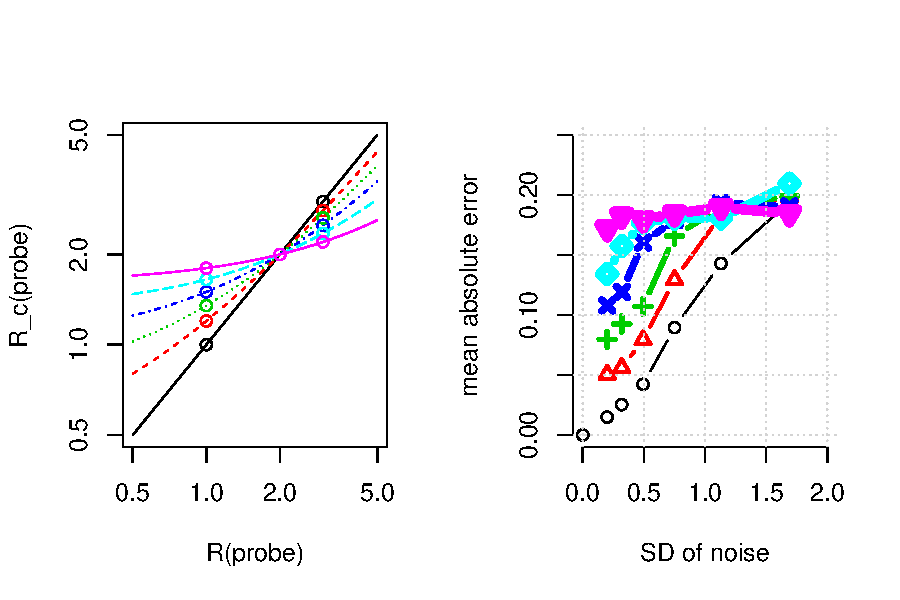
\includegraphics[width=6in]{contam.pdf}
\label{fig:contam_stat}
\caption{Higher contamination are more prone to noise}
\end{figure}

\begin{figure}
\centering
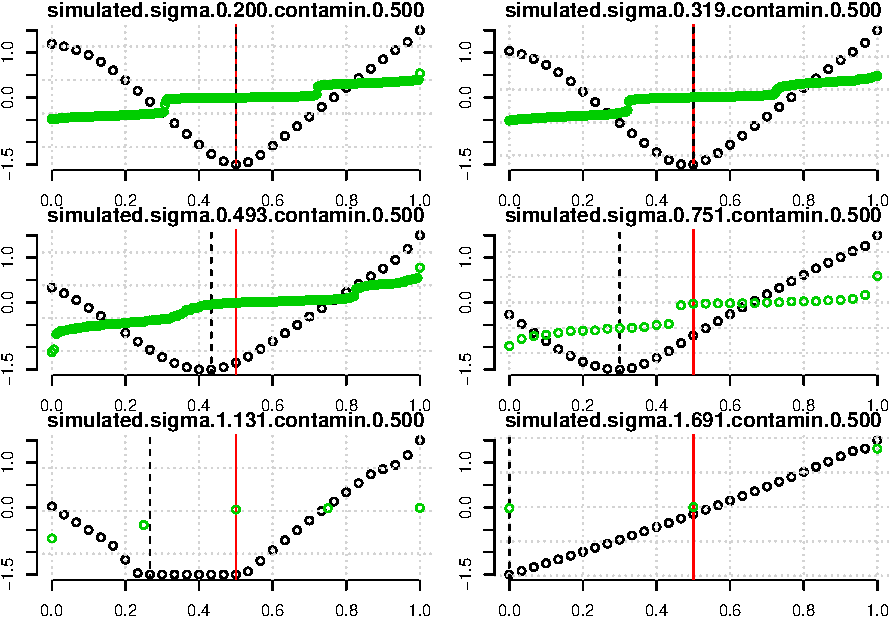
\includegraphics{copynumber_files/figure-latex/contam_est-1.pdf}
\caption{\label{fig:contam_est} Estimating conatmination level by
minimising MAE. Red: Actual contamination ratio (c-ratio) Black:
estimated c-ratio}
\end{figure}

\begin{figure}
\centering
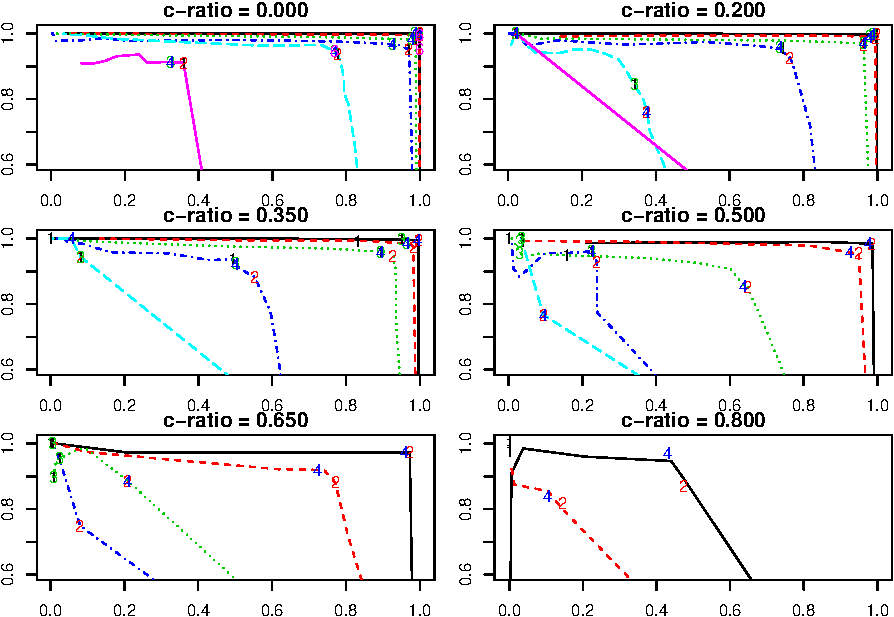
\includegraphics{copynumber_files/figure-latex/plot__PR2-1.pdf}
\caption{\label{fig:eval_thres2} Evaluation of different threshold.
Coloured by increasing noise level)}
\end{figure}

\paragraph{Conclusion}\label{conclusion}

We have tested the efficacy of CBS algorithm using a simulated dataset
and assessed its performance under different noise level. Furthermore,
we suggested to use cluster-based thresholding to improve the
copy-number calling. We then go on to adapt this methodology under a
normal cell contamination by incorporating an estimator for
contamination, but uncovering the unfortunate fact that the weakness in
contamination estimation is destroying the whole algorithm. However, we
highlight the usefulness of both naive thresholding and cluster-based
thresholding, given that the contamination ratio. Thus the whole system,
will benefit from a robust estimator for contamintation ratio.

\begin{verbatim}
tpbs = pbs[1:10]
i = 1
(probes[i] <= tpbs[-1]) & (probes[i] > tpbs[-length(tpbs)]) 

# probes_mat = matrix(probes,ncol = 1)
probe = probes[1]

# copy_number = (probes_mat <= segEND[-1]) & (probes_mat >= segEND[-length(segEND)])
# copy_number%f%dim
# copynumber
\end{verbatim}

References: 1. Adam B. Olshen, E. S. Venkatraman, Robert Lucito, Michael
Wigler; Circular binary segmentation for the analysis of array based DNA
copy number data, Biostatistics, Volume 5, Issue 4, 1 October 2004,
Pages 557--572,


\end{document}
